\subsection{Whisper}

Whisper~\cite{Radford_Kim_Xu_Brockman_McLeavey_Sutskever_2022} est un modèle de \gls{asr} proposé par OpenAI.
À l'instar de Wav2Vec, son architecture comporte un \gls{cnn} et un transformeur.
Cependant, contrairement à Wav2Vec, l'entrée n'est pas la forme temporelle du signal audio.
Il s'agit plutôt de représentation spectrale (voir Figure~\ref{fig.whisper}).
Whisper utilise un encodage positionnel sinusoïdal pour l'audio (similaire à~\cite{attention})
et un encodage positionnel appris pour le texte (voir section~\ref{sec.transformers}).

\begin{figure}[hbt]
    \centering
    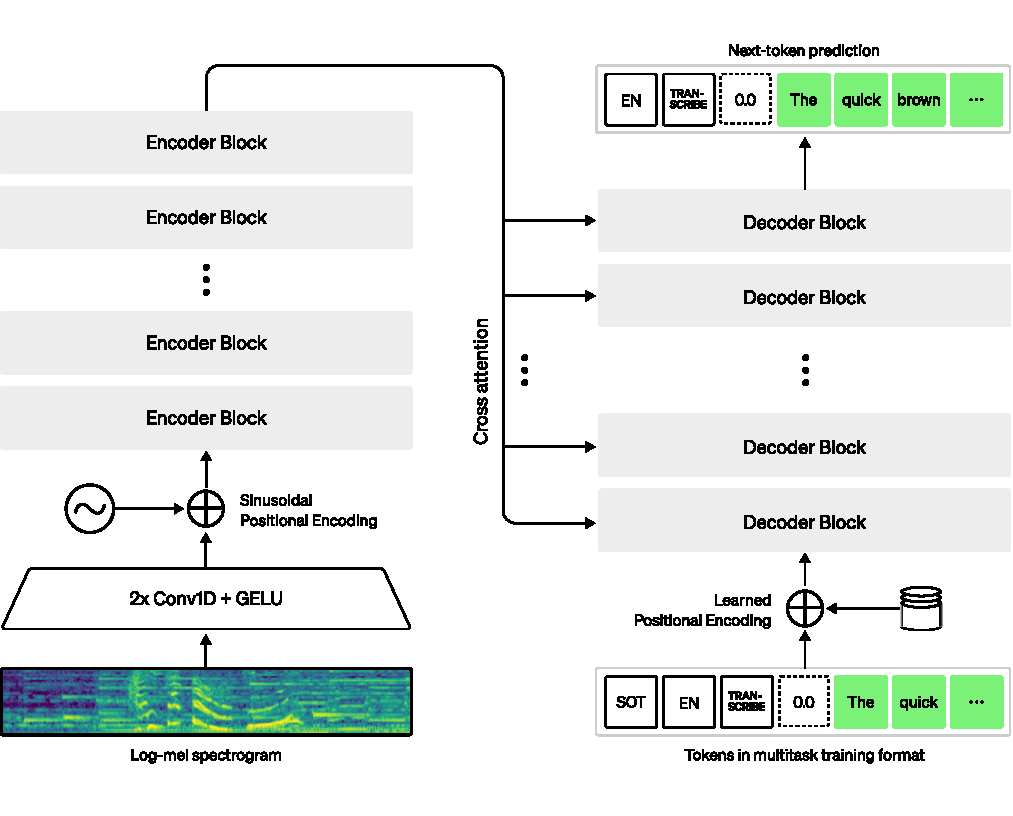
\includegraphics[width=.5\linewidth]{assets/pdf/whisper.pdf}
    \caption[Architecture de Whisper.]
    {Architecture de Whisper~\cite{Radford_Kim_Xu_Brockman_McLeavey_Sutskever_2022}.}
    \label{fig.whisper}
\end{figure}